\section{Assignment 3}

\subsection{Introduction}
\todo{Introduction to the assignment}

\subsection{autonomous and non-autonomous systems}
\begin{figure}[H]
    \centering
    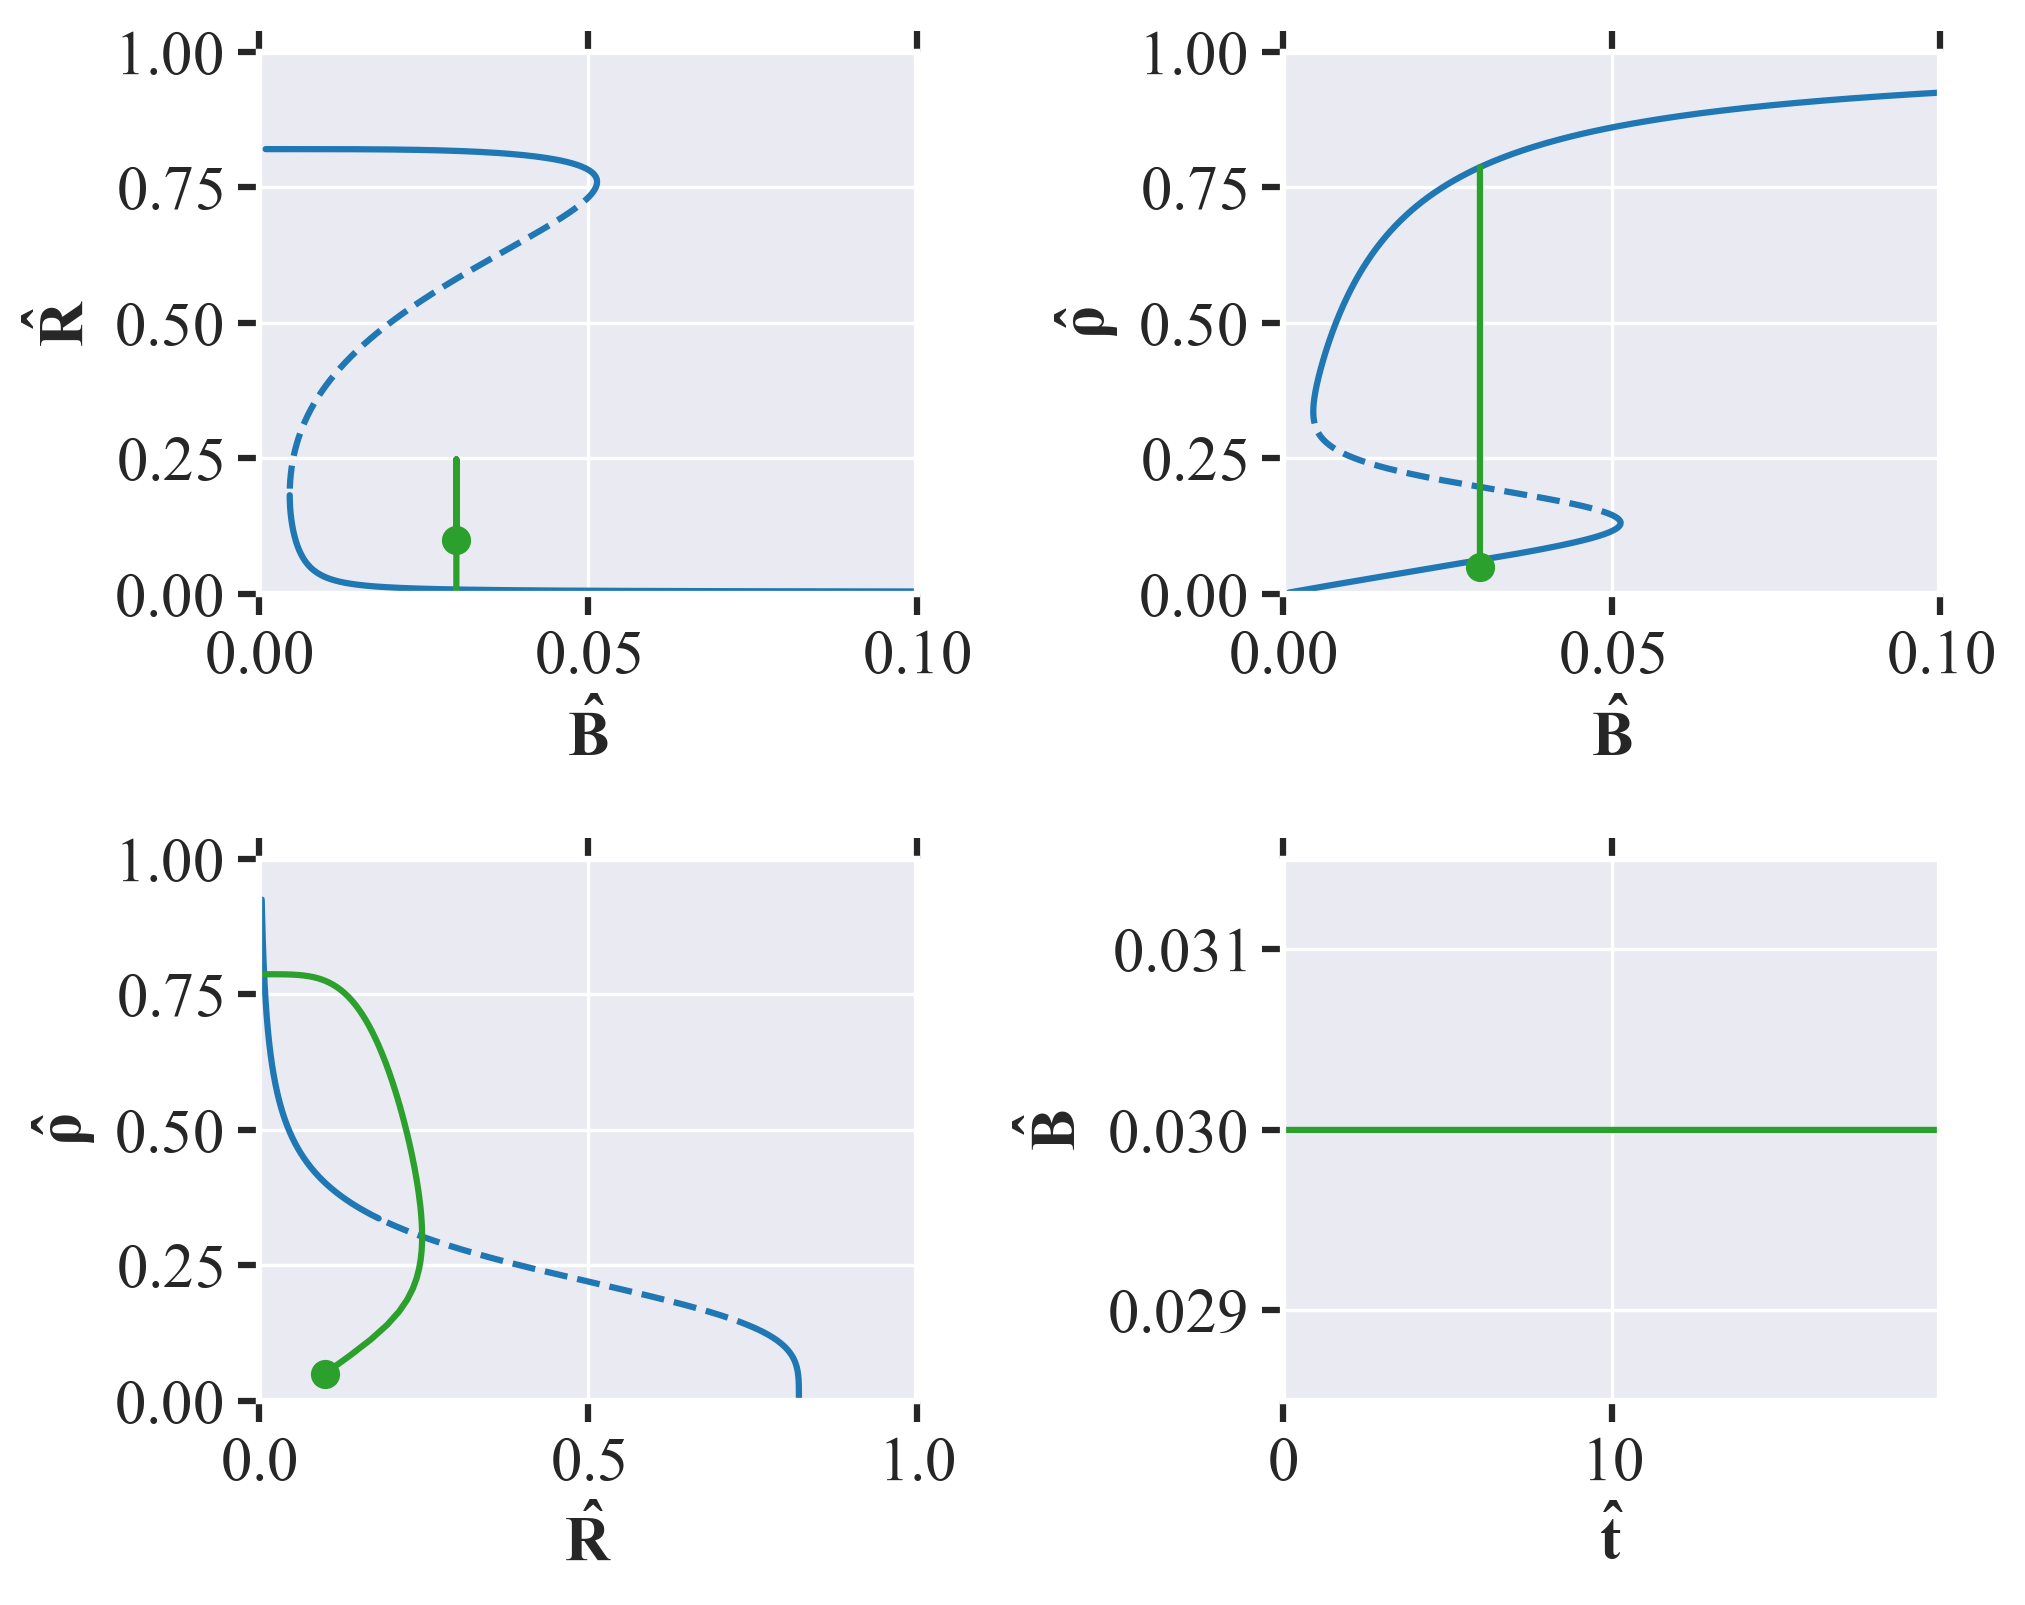
\includegraphics[width= \textwidth]{figures/cell_biology_R0=0.3_rho0=0.16_deltaR=1_n=4_Bmax=0.04_eps=0.0.png}
    \caption{Figure of the continuation of \textbf{top left:} $(\hat{R}, \hat{B})$ and \textbf{top right:}, $(\hat{\rho}, \hat{B})$, \textbf{bottom left:} phase space $(\hat{rho}, \hat{R})$ and 
    \textbf{bottom right:} $\hat{B}$ against time.}
    \label{fig:cell_biology_ex1}
\end{figure}

\subsection{Conclusion}
\todo{Conclusion to the assignment}